In $e^+e^-$-, $pp$- oder $p\bar{p}$-Kollisionen wird in den zugehörigen Detektoren der Spurverlauf
(oft) im Magnetfeld gemessen. Der Impuls der Teilchen kann dann aus der Sagitta berechnet werden
(s. Abb. \ref{sagitta}).

\begin{figure}[H]
	\centering
	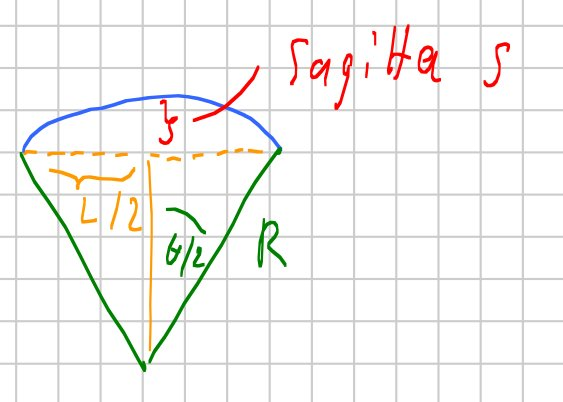
\includegraphics[width=0.5\textwidth]{sagitta.jpg}
	\caption{	 ???}
	\label{sagitta}
\end{figure}

\[S= R-\sqrt{R^2-\left(\frac{L}{2} \right)^2} = R-R\cdot\text{cos}\frac{\Theta}{2}\approx R\cdot
\frac{\Theta^2}{f???} \]

Mit $\Theta = e\cdot B\cdot L/p$ folgt

\[S= \frac{e\beta\cdot L^2}{f???p}~~~~~~\text{mit}~~~p=e\cdot\beta\cdot R. \]

Wird die Teilchentrajektorie im Magnetfeld an $N$ äquidistanten Punkten gemessen, so ist der
Impulsfehler aufgrund der Ortsmessgenauigkeit $\sigma(x)$ durch die sogenannte Glückstern-Formel
gegeben:

\[ \frac{\sigma^{\text{Ort}}(p)}{p} = \frac{\sigma(x)}{0{,}3\cdot\beta L^2}\cdot
\sqrt{\frac{720}{N+4}}\cdot p \]

mit den Einheiten $\sigma(x)\left[\text{mm} \right]$, $L\left[\text{m} \right]$,
$\beta\left[\text{T} \right]$ und $p\left[\text{GeV/c} \right]$.
\\
Da die $N$ Punkte äquidistant über $L$ verteilt sind, zeigt sich

\[ \frac{\sigma^{\text{Ort}}(p)}{p} \sim \frac{1}{L^{5/2}}\cdot \frac{1}{\beta}\cdot p \]

Das heißt eine Vergrößerung von $L$ verbessert die Impulsauflösung besser als ein stärkeres
Magnetfeld. Die Vielfachstreuung trägt auch bei solchen Detektoren

\[\frac{\sigma^{\text{up???}}(p)}{p} = \frac{0{,}05}{\beta \cdot L}\cdot \sqrt{\frac{1{,}43\cdot
L}{x_0}} \]

bei. 
\\
Bisher wurde nur der Impuls senkrecht zu $\beta$ bestimmt. Interessant ist aber der Gesamtimpuls
$p$. 

\begin{figure}[H]
	\centering
	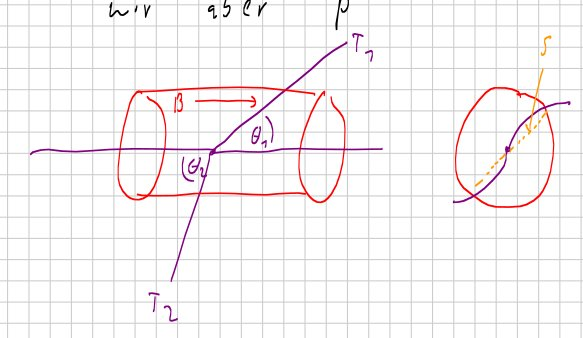
\includegraphics[width=0.5\textwidth]{collider1.jpg}
	\caption{	 ???}
	\label{collider1}
\end{figure}

Durch die Messung von $\Theta_1$ und $p_T$ (Impuls in der Transversalebene zum Magnetfeld) folgt

\[p=\frac{p_T}{\text{sin}\,\Theta} .\]

\begin{figure}[H]
	\centering
	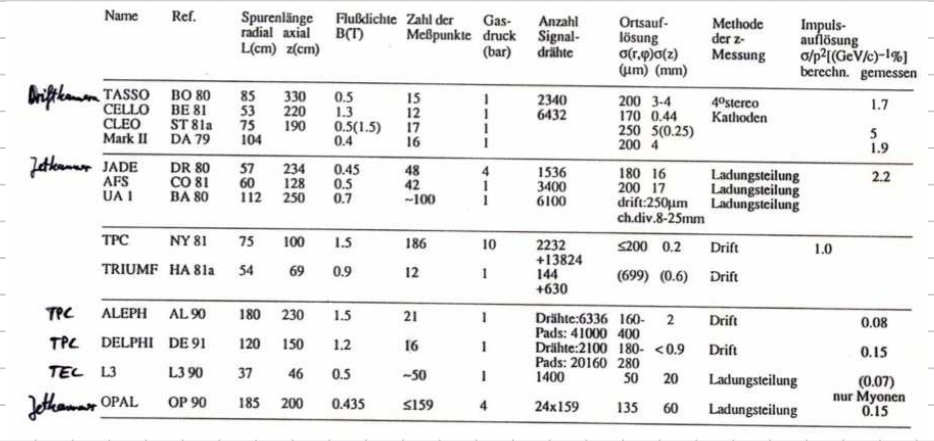
\includegraphics[width=0.5\textwidth]{collidertab.jpg}
	\caption{	 ???}
	\label{collidertab}
\end{figure}